В главе описан порядок разработки  педагогических инструментов, использующих интеллектуальных ассистентов. Глава разделена на секции 
\begin{itemize}
    \item анализ существующих инструментов повышения эффективности труда с использованием искуственного интеллекта
    \item разработка образовательных игр, обучающих использованию ассистентов 
\end{itemize}


\begin{figure}[h]
    \centering
    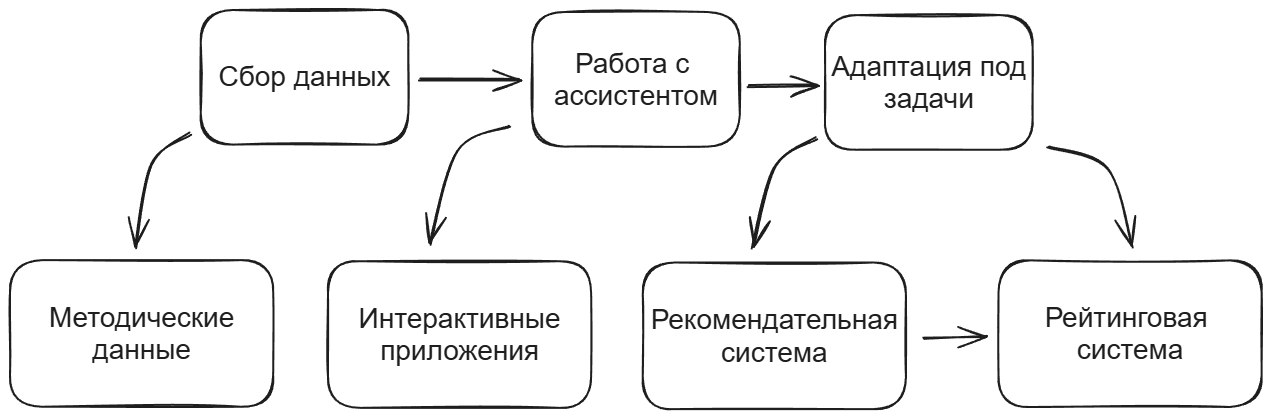
\includegraphics[width=0.5\textwidth]{assets/work/overview/plan.excalidraw.png}
    \caption{Этапы работы}
    \label{chess}
\end{figure}

Исходным этапом работы являлось создание подготовка задач, составленных с помощью 

